\section{Analysis Workflow Overview}
\label{sec:analysis-workflow-overview}

\section{Gammapy package}
\label{sec:gammapy-package}

The \gammapy package is structured into multiple sub-packages which mostly
follow the stages in the data reduction workflow.

\subsection{Overview}
\label{ssec:overview}
\begin{figure*}[t]
	\centering
	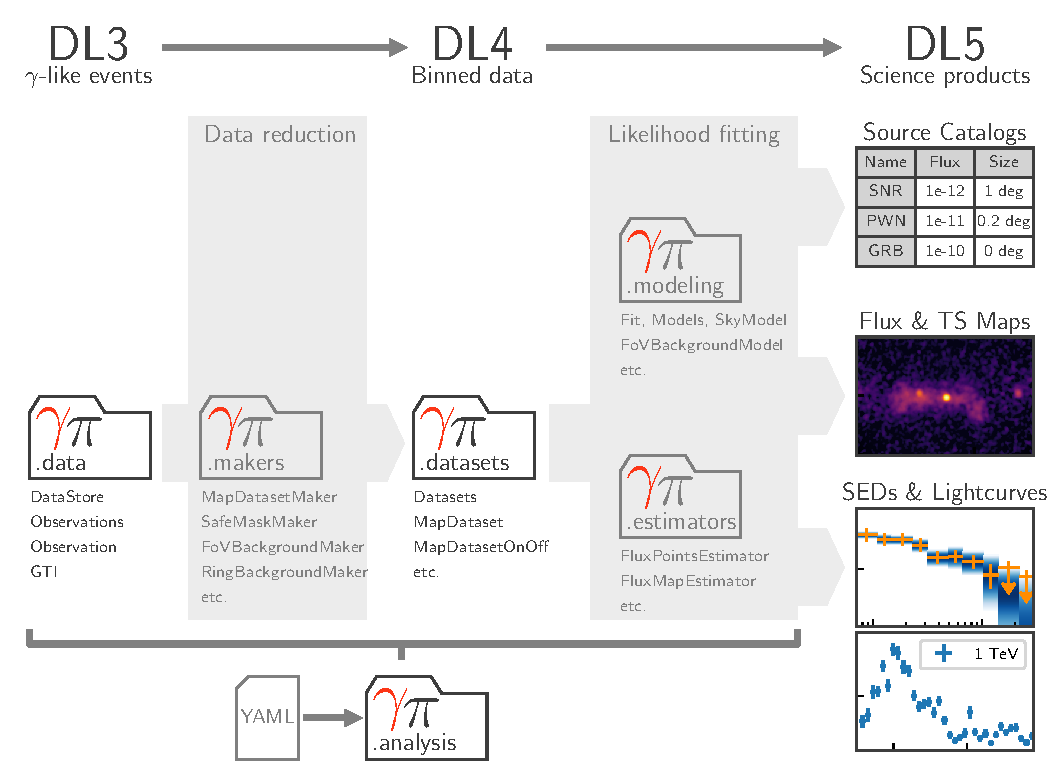
\includegraphics[width=1.\textwidth]{static/data-flow-gammapy}
	\caption{
		Gammapy sub-package structure and data analysis workflow. }
	\label{fig:workflow} \end{figure*}

\subsection{gammapy.data}
\label{ssec:gammapy-data}
The \verb|gammapy.data| sub-package provides access to DL3 level data and
observation handling.

\begin{figure}

	\import{code-examples/generated/}{gp_data}

	\caption{Using gammapy.data to access DL3 level data with a DataStore}
	\label{fig*:minted:gp_data}
\end{figure}

\subsection{gammapy.makers}
\label{ssec:gammapy-makers}
\todo{Regis Terrier}
Data reduction

\begin{figure}
	\import{code-examples/generated/}{gp_makers}

	\caption{Using gammapy.data to access DL3 level data}
	\label{ig*:minted:gp_makers}
\end{figure}

\subsection{gammapy.datasets}
\label{ssec:gammapy-datasets}
\todo{Atreyee Sinha}
DL4 level data

\begin{figure}

	\import{code-examples/generated/}{gp_datasets}
	\caption{Using gammapy.data to access DL3 level data with a DataStore}
	\label{fig*:minted:gp_datasets}
\end{figure}

\subsection{gammapy.modeling
\label{ssec:gammapy-modeling}
\todo{Quentin Remy}
Models and fitting

\begin{figure}
	\import{code-examples/generated/}{gp_models}
	\caption{Using gammapy.modeling.models}
	\label{fig*:minted:gp_models}
\end{figure}

\subsection{gammapy.estimators}
\label{ssec:gammapy-estimators}
\todo{Axel Donath}
Estimators

\subsection{gammapy.visualisation}
\label{ssec:gammapy-visualisation}
Plotters etc.

\subsection{gammapy.analysis}
\label{ssec:gammapy-analysis}
\todo{Jose Enrique writes this...}
High level analysis API

\subsection{gammapy.astro}
\label{ssec:gammapy-astro}
Dark matter models, source population modelling

\subsection{gammapy.data}
\label{ssec:gammapy-data}
\todo{Cosimo Nigro}

\subsection{gammapy.catalog}
\label{ssec:gammapy-catalog}
Gamma-ray catalog access

\begin{figure}
	\import{code-examples/generated/}{gp_catalogs}
	\caption{Using gammapy.catalogs}
	\label{codeexample:data}
\end{figure}

\subsection{gammapy.maps}
\label{ssec:gammapy-maps}
\todo{Laura Olivera-Nieto}
The \verb|gammapy.maps| sub-package provides classes for representing pixelized
data structures with at least two spatial dimensions representing a set of
coordinates or a region on a sphere. In addition it allows to handle and
arbitray  number of non-spatial data axes, such as time or energy.

It provides a uniform API for WCS, HEALPix and region based data structures.

\begin{figure}
	\import{code-examples/generated/}{gp_maps}
	\caption{Using gammapy.data to access DL3 level data with a DataStore}
	\label{codeexample:data}
\end{figure}

\subsection{gammapy.irf}
\label{ssec:gammapy-irf}
\todo{Fabio Pintore}
IRF classes

\subsection{gammapy.stats}
\label{ssec:gammapy-stats}
\todo{Regis Terrier}
Statistics methods

\subsection{gammapy.utils}
\label{ssec:gammapy-utils}
Utility functions...

Outline: * List typical analysis use cases * Can use from Python and Jupyter ->
show Figure with Jupyter notebook here. * Gammapy code structure * How Numpy
and Astropy is used

Figures: * Add a Figure showing dataflow in a typical application DL3 at the
top, spectrum, map, lightcurve, fit results at the bottom. Mention major
classes in between (DataStore, EventList, Map, MapMaker, MapFit, …) * Probably
not: Figure showing sub-packages and how they relate (gammapy.data and
gammapy.irf at the base, then gammapy.maps, etc. * The code example Figure how
to make a counts map, to explain how the package works.
